%-------------------------------------------------------------------------------
\section{Implementation}
%-------------------------------------------------------------------------------

%-------------------------------------------------------------------------------
\section{Evaluation}
%-------------------------------------------------------------------------------
\iffalse

write something like the 3 questions that we want to answer
followed by subsections that say what the goal of this section is, the setup of the experiment, and the results

obladi/zyzzyva/tapir eval structure:
1. Questions: What advantage does PO replication bring. What price does Indicus pay for BFT. How does it perform under contention. How does it perform under failures.
2. Experiment setup and Testbed setting
3. Implementation (what protobuf, Use Sha256 for hash, ECDSA for scheme (256 bit prikey, crypopp library https://www.cryptopp.com/) and baselines: NoPO (uses same spec execution and TSO, but AB for validation ordering)
4. Workloads
5. Q1 impact of partial order
6. Q2 comparison to crash failure (overhead of bft
7. Q3 abort rates
8. Q4 performance under failures

Indicus3 eval missing. We do not include it because it violates to byzn independence when using dependencies. We could in theory eval it without deps to just show partial order impact. If clients are not byzantine it doesnt matter.
\fi




\fs{Question: Is clock skew something we need to explicitly handle? Clock sync etc across machines?}

\fs{CPU vs Network bottleneck? How does this affect our results}

Our evaluation seeks to answer the following questions:
\begin{itemize}
  \item How do the throughput and latency of \sys{} compare to the
    state-of-the-art distributed replicated transactional key-value
    stores?
  \item What are the overheads of providing byzantine fault tolerance over
    crash fault tolerance?
  \item How is the commit rate affected by the choice of concurrency control?
  \item What is the tradeoff between leader-based replication and quorum-based
    replication? CHANGE TO: total order vs no-order/partial order. Gain of abolishing TO
  \item How does \sys{} perform when clients or replicas exhibit Byzantine
    behavior?
\end{itemize}

\paragraph{Implementation and Baselines.} We implemented our prototype of \sys in TODO lines of C++ code. To evaluate the overheads of byzantine fault tolerance, we compare against TAPIR\cite{zhang2015tapir}, a state of the art distributed transaction system for the crash failure model, that like \sys sidesteps total-order replication. In order to facilitate a fair comparison we build \sys atop TAPIR communication layer, and extend it to provide authentication. We use SHA256 Hash functions and ECDSA signatures provided by the cryptopp library (https://www.cryptopp.com/). Further, we implement a strawman BFT baseline NoPO that, unlike \sys, (optionally) uses naive Optimistic Concurrency control, and relies on PBFT cite() to provide totally ordered broadcast for the Validation layer. (We use signatures instead of MAcs for PBFT. But ECDSA is much more efficent than RSA, and cpu should not be the bottleneck?) NoPO maintains \sys 's speculative Execution structure in order to offer interactive transactions. fs{if we moved the speculative execution to a single replica that processes reads and buffers writes then it would simulate BFT-DUR }. \fs{Lastly, we modify Hyperledger Fabric, a popular enterprise-ready permissioned Blockchain solution, to process Online Transactional Processing (OLTP) workloads (instead of smart contracts) in order to facilitate a comparison with a state of the art blockchain. To do so, we replace the Simulation layer with NoPO's speculative execution.}

\paragraph{Workloads.} We evaluate the performance of \sys using the TPC-C and Smallbank workloads to simulate realistic Online Transaction Processing (OLTP) applications. TPC-C simulates the business logic of an e-commerce vendor operating multiple warehouses, while Smallbank simulates a small-scale banking application that allows for transfers, deposits, and withdrawals. Additionally, we use the YCSB workload generator for our microbenchmarks in order to simulate random distributions of read/write requests.

\paragraph{Setup.} We run all our experiments using CloudLab machines (TODO: specs), in both in-datacenter (LAN) and cross-datacenter (WAN) environments. For WAN settings, we respectively place 1/3 of replicas in geographic regions USA, Europe, and Asia; Figure X. shows single-hop message-delays. (TODO: latencies in LAN and WAN - maybe do only WAN).

\paragraph{Methodology.} Our reported results are based on experiments run by closed loop clients for several minutes, and exclude measurements during warm-up (first X fraction) and cool-down (last X fraction).

\subsection{Applications}

\begin{figure}
  Scatter Plot\\
  X-axis: throughput (committed new order transactions per second)\\
  Y-axis: latency (median)\\
  Series: Indicus, TAPIR, OCC+PBFT, Hyperledger\\
  Workload: TPC-C\\
  Setup: WAN, 3 shards / groups\\
  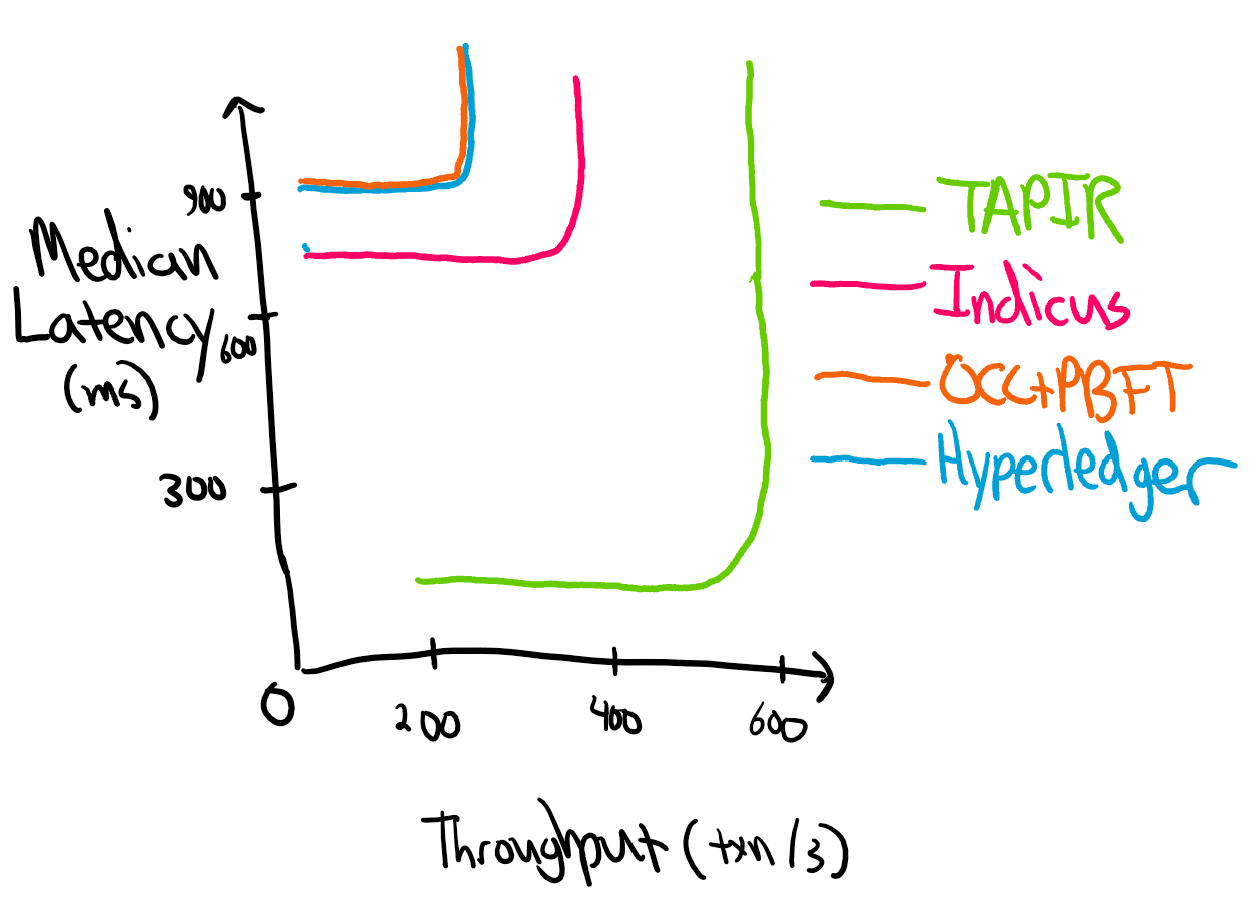
\includegraphics[width=\columnwidth]{figures/eval/tpcc-tput-lat.png}
  \caption{Throughput versus latency of \sys{} and baselines for the TPC-C
  workload in a wide-area network deployment.}
  \label{fig:tpcc-tput-lat}
\end{figure}

We measure the throughput and median latency of \sys{} and all baselines with the
industry standard TPC-C benchmark (Smallbank too?). Each system is configured to tolerate $f=1$
failures and replicas are deployed across a WAN. Clients are co-located with
replicas in each geographic region, so the round trip time between a client and
its nearest replica is much less than the wide-area network round trip time when
all replicas are correct and responsive. The data is partioned across
three groups of replicas (3 shards). Figure~\ref{fig:tpcc-tput-lat} shows the results.

TAPIR achieves the lowest median latency when not saturated because reads only
need to be executed at the nearest replica and it often commits transactions in
a single round trip on the fast path of its commit protocol.

In order to avoid maliciously stale execution, Hyperledger, OCC+PBFT, and \sys{} require reads to be executed at $f+1$ replicas, and hence requires at least one wide-area network round trip
to the second (or third) nearest replica. When reading from a single replica, performance improves by TODO, at the risk of higher abort rate and lack of responsiveness (need to send to f+1 to receive 1).

Once the execution phase is complete,
\sys{} often commits in a single round trip on the fast path to all $5f+1$
replicas as in TAPIR. Hyperledger and OCC+PBFT require additional message delays
because their commit protocols are a) routed via a leader replica at each shard and b) mandate additional coordination to enforce consistency. (Would need to do Zyzzyva to make only a leader bottleneck)

TAPIR moreover achieves the highest throughput before saturation because it does not
require expensive signature computations and validation of proofs. \sys{} achieves
better throughput than Hyperledger and OCC+PBFT as proposal load is balanced across client coordinators instead of single primary replica that must sequence every transaction per shard ( as is the case with the leader replicas in Hyperledger
and OCC+PBFT).


\subsection{Microbenchmarks}


\begin{figure}
  Bar Graph\\
  Y-axis: throughput at saturation (committed transactions per second)\\
  Workload: YCSB+T, moderate skew\\
  Series: Indicus (no proofs, no signatures), Indicus (proofs, no signatures),
    Indicus (no proofs, signatures), Indicus (full), TAPIR\\
  Setup: WAN, 3 shards / groups\\
  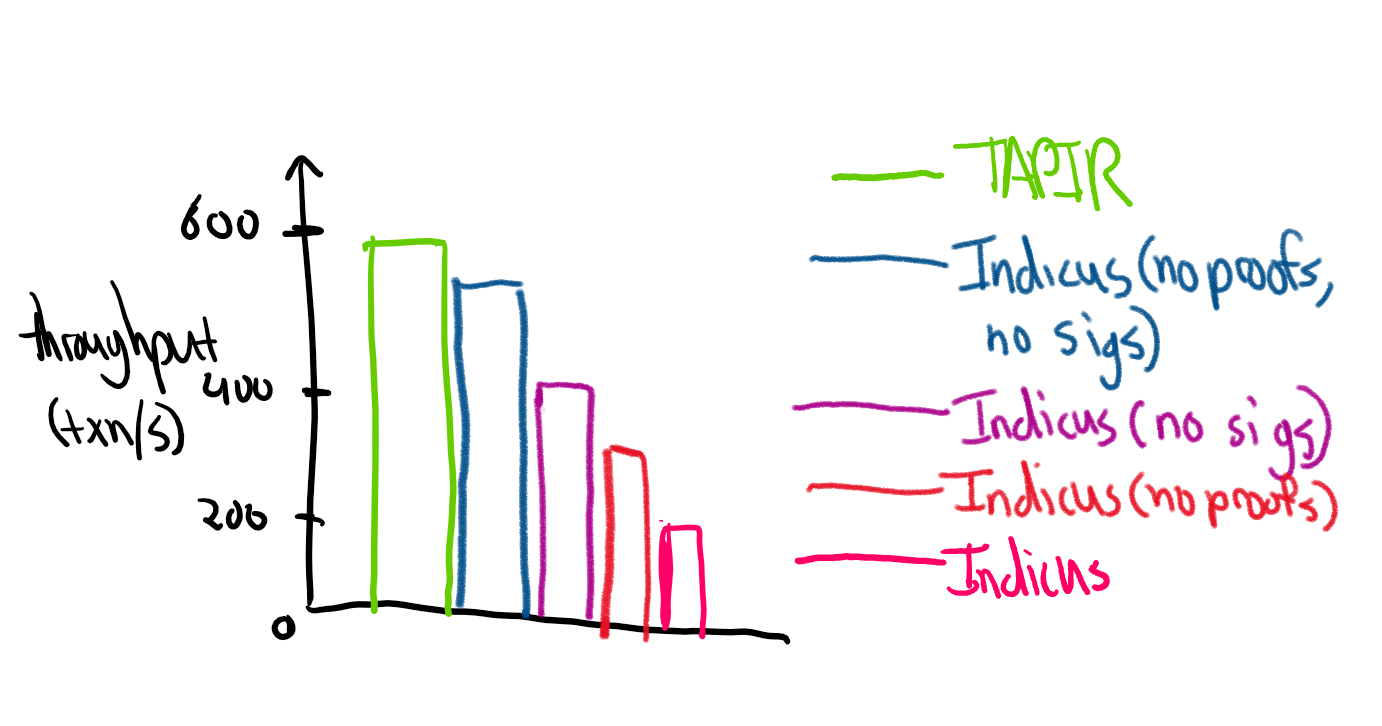
\includegraphics[width=\columnwidth]{figures/eval/bft-overhead-tput.png}
  \caption{Throughput of \sys{} with increasing amounts of Byzantine
  ``protection'' for fixed YCSB+T workload.}
  \label{fig:bft-overhead-tput}
\end{figure}

\paragraph{BFT Overheads.} We measure the maximum throughput of \sys{} and TAPIR with the YCSB+T workload at moderate skew in order to quantify the performance overhead of tolerating byzantine failures.
Figure~\ref{fig:bft-overhead-tput} shows the results.

Indicus with no proofs and no signatures comes within 10\% of the throughput of
TAPIR. This is because Indicus' commit protocol exchanges around the same
number of messages per replica as TAPIR's commit protocol, with
transactions committing after either one round trip to every replica or after
two round trips to all honest replicas.  TAPIR still achieves slightly
better throughput because reads are only executed by a single replica whereas in
Indicus, reads are executed by $\geq f+1$ replicas. 

\fs{Need to evaluate impact of RQS: Compare with just 1 read, f+1 reads, or >3f+1 (for read locks). Create more read/write conflicts and see whether read locks actually help.}

Indicus with signatures and no proofs achieves a lower maximum throughput than
Indicus with no signatures and no proofs because signature computations are
expensive.

Similarly, the computation required to serialize, deserialize, and validate
proofs reduces the throughput of Indicus with no signature and proofs relative
to Indicus with no signatures and no proofs and TAPIR.

Indicus with both signatures and proofs achieves the lowest maximum throughput.
In total, tolerating Byzantine failures imposes about a 75\% throughput overhead
for this workload.

\begin{figure}
  Bar Graph\\
  X-axis: grouped by geographic region\\
  Y-axis: latency at fixed non-saturated load (average + 25th and 75th percentiles)\\
  Workload: YCSB+T, moderate skew\\
  Series: Indicus, TAPIR\\
  Setup: WAN, 3 shards / groups\\
  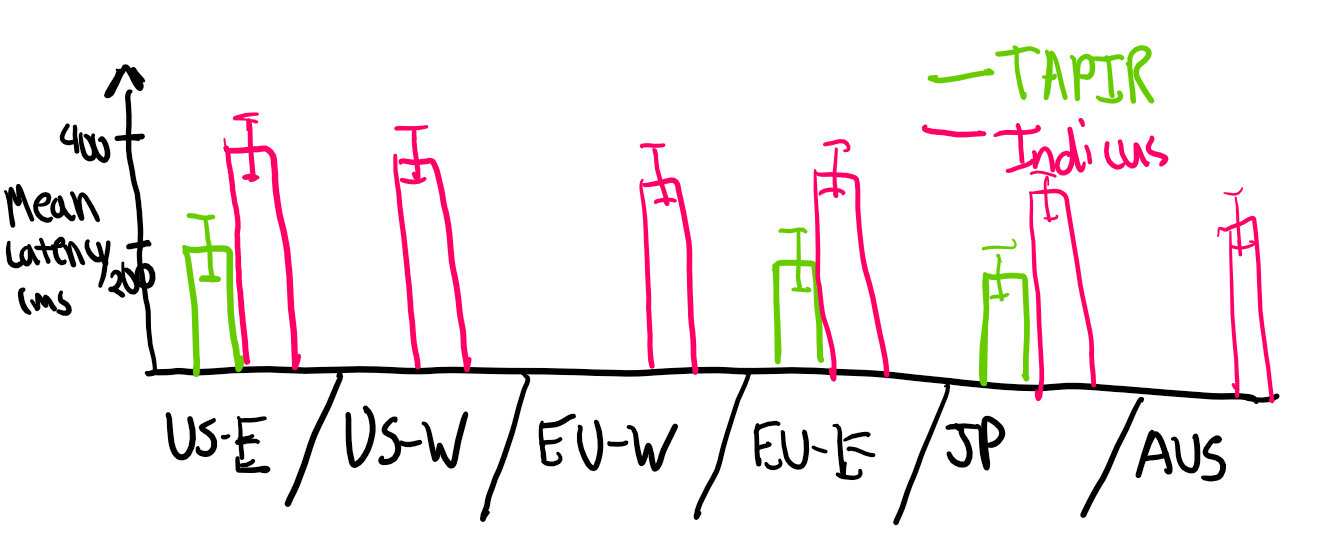
\includegraphics[width=\columnwidth]{figures/eval/bft-overhead-lat.png}
  \caption{Region-by-region latency of \sys{} and TAPIR for fixed YCSB+T workload.}
  \label{fig:bft-overhead-lat}
\end{figure}

Figure~\ref{fig:bft-overhead-lat} shows the latency overheads of tolerating
Byzantine failures. Using the same workload as before, we measure the average,
first quartile, and third quartile latencies. 

\sys{} has higher latency than TAPIR in all geographic regions because its
reads must be executed by $f+1$ replicas instead of just a single replica. This
requires reads to be sent across the wide-area network, which increases total
transaction latency in proportion to the number of reads in the transaction.

\begin{figure}
  Scatter Plot\\
  X-axis: Zipfian parameter\\
  Y-axis: Abort Rate (1 - committed / attempts)\\
  Workload: YCSB+T\\
  Series: Indicus, TAPIR\\
  Setup: WAN, 3 shards / groups\\
  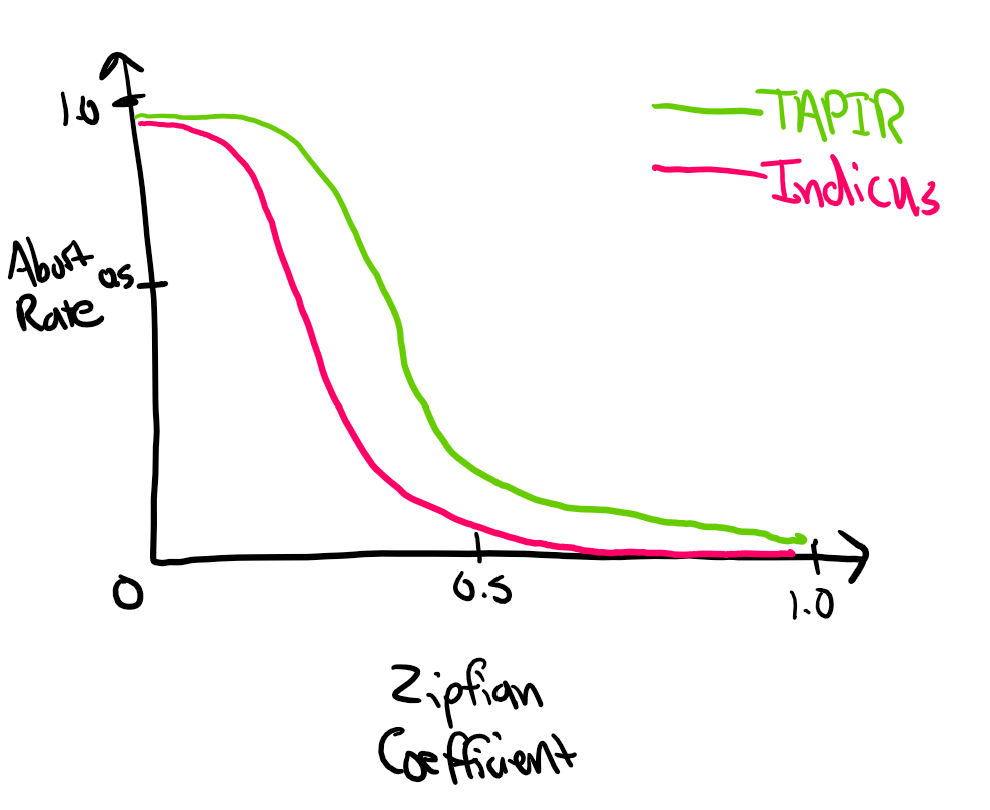
\includegraphics[width=\columnwidth]{figures/eval/bft-overhead-aborts.png}
  \caption{Abort rate of \sys{} and TAPIR with increasing skew.}
  \label{fig:bft-overhead-aborts}
\end{figure}

Figure~\ref{fig:bft-overhead-aborts} shows the commit rate overhead of tolerating
Byzantine failures. It shows the abort rate of transactions from the YCSB+T
workload with increasing contention. 

Because \sys{}'s execution phase takes longer than TAPIR, there is a larger
window during which conflicting transactions can overlap. This directly leads
to more aborts.

\begin{figure}
  Scatter Plot\\
  X-axis: Zipfian parameter\\
  Y-axis: Abort Rate (1 - committed / attempts)\\
  Workload: YCSB+T\\
  Series: Indicus+OCC, Indicus+MVTSO-RTS-DEP, Indicus+MVTSO-DEP, Indicus+MVTSO\\
  Setup: WAN, 3 shards / groups\\
  \caption{Abort rate of \sys{} with different types of concurrency control
  increasing skew.}
  \label{fig:cc-aborts}
\end{figure}

\paragraph{Concurrency Control.} Figure~\ref{fig:cc-aborts} shows how the choice of concurrency control in
\sys{} affects the abort rate of transactions under increasing levels of 
contetion.

Indicus+OCC uses basic OCC validation that disallows concurrenct conflicting
transactions from committing. Indicus+MVTSO improves (reduces the number of
aborts) on this by allowing transactions to read from older versions and by
allowing concurrent conflicting write transactions to commit if their assigned
timestamps match their validation orer at each shard.

Indicus+MVTSO+RTS further improves abort rate by reducing the size of the window
during which transactions execution overlaps. 

Indicus+MVTSO+RTS+DEP improves on this even further by allowing transactions to
read uncommitted writes. This comes at the risk of cascading aborts.

\begin{figure}
  Scatter Plot\\
  X-axis: throughput (committed transactions per second)\\
  Y-axis: latency (median)\\
  Series: Indicus+OCC, OCC+PBFT\\
  Workload: YCSB+T\\
  Setup: WAN, 3 shards / groups\\
  \caption{Throughput versus latency of \sys{} w/ simple OCC check and
  OCC+PBFT in a wide-area network deployment.}
  \label{fig:to-vs-po-tput-lat}
\end{figure}

\paragraph{Enforcing partial order} Figure~\ref{fig:to-vs-po-tput-lat} shows the overhead from the leader-based
OCC+PBFT relative to the quorum-based \sys{}. Latency is higher because leader-based
protocols require redundant wide-area round trips during the validation phase. Moreover, the total order requirment implies that validation must wait for all previously sequenced operations to complete (instead of happing as soon as it arrives), resulting in idle times.
Throughput is lower because the leader of each shard processes every transaction
that touches the shard whereas in quorum-based protocols, the processing load 
may be spread equally across all replicas in the shard (coordination overheads are delegated to clients in fact). (Throughput is also affected because of the sequential waits?)
\fs{Need to add batching for PBFT?}
(An optimization we do not currently explore is parallelizing validation: This could be done in Indicus by acquiring locks and spawning a thread that takes care of it)
PBFT has low throughput because of all to all communication. We use a second variation where the primary acts as collector and broadcast channel for all communication. This decreases message complexity (signatures stay quadratic), but increases latency.

\iffalse
\paragraph{Leaders vs. Quorums.} Figure~\ref{fig:to-vs-po-tput-lat} shows the overhead from the leader-based
OCC+PBFT relative to the quorum-based \sys{}. Latency is higher because leader-based
protocols require redundant wide-area round trips during the validation phase.
Throughput is lower because the leader of each shard processes every transaction
that touches the shard whereas in quorum-based protocols, the processing load 
may be spread equally across all replicas in the shard.
\fi

\subsection{Failures}

\begin{figure}
  Scatter Plot\\
  X-axis: time (since start of experiment)\\
  Y-axis: throughput (committed transactions per second)\\
  Series: Indicus\\
  Workload: TPC-C\\
  Setup: WAN, 3 shards / groups, Byzantine replica failure at midway point of
  experiment.\\
  \caption{Throughput over time of \sys{}. A replica exhibits Byzantine
  behavior at time $t=x$.}
  \label{fig:failure-replica-tot}
\end{figure}

\begin{figure}
  Scatter Plot\\
  X-axis: time (since start of experiment)\\
  Y-axis: throughput (committed transactions per second)\\
  Series: Indicus\\
  Workload: TPC-C\\
  Setup: WAN, 3 shards / groups, Byzantine clients attack system at midway point
  of experiment.\\
  \caption{Average latency over time of \sys{}. A subset of clients exhibit
  Byzantine behavior at time $t=x$.}
  \label{fig:failure-clients-lot}
\end{figure}

Lastly, we evaluate the performance of \sys during failures. Concretely, in Figure \ref{fig:failure-replica-tot} we show how throughput is affected under single replica failure. \sys must resort to the Slow Path for Validation, and reads during execution must wait for an additional WAN result (if the faulty replica was one of the nearest). Hence latency increases, while throughput decreases due to the increased load (p2 messages, and more reads).
(how does this stack up against pbft that does not use a fast path?)

Next, we evaluate the throughput of \sys under client failures. We simulate client failure by letting a subset of clients time out (or equivocate) during Execution, Validation, and Writeback. Lack of participation during Execution affects throughput since conflicting tx might abort. 
Omission/Equivocation during Validation and Writeback invokes the Fallback protocol. This adds additional latency overhead for the affected transactions, and hurts throughput since more messages are being sent... But it does not bring throughput to 0, because the system stays live for all unaffected objects. Moreover, the single shard logging optimization helps improve throughput because only a single shard is involved in the fallback.



\fs{Optional paragraph: How does the system behave when scaling number of shards or shard size}

%%%%%%%%%%%%%%%%%%%%%%%%%%%%%%%%%%%%%%%%%%
\iffalse
Questions:
\begin{itemize}
  \item Are there any experiments where we explcitily want to measure behavior in LAN?
  \item Hyperledger uses stored procedures/one-shot transactions - how do we compare this to Indicus? Do we use the read-only + conclusory transaction strategy? Or rewrite workloads as one-shot for Hyperledger?
  \item 
\end{itemize}

Question: Is clock skew something we need to explicitly handle? Clock sync etc across machines?

Plan for the evaluation:
1) Questions and experiments that answer those.
  1. compare against state of the art: Tapir, vs Hyperledger (our version)
  

- Need TPC-C
- Try to get Hyperledger to run
- If benefit of partial order is worse than engineering optimization its not worth doing. 
- Could add smart contract layer (like ethereum evm) on top of ours(? probably dont want this)

Is there code that inputs smallbank into hyperledger smart contracts api. ?


2) Which experiments and write the sections on what we expect. What do the graphs look like.


Headline graph: Show performance compared to TApir, hyperledger, occ+pbft.

\subsection{Experiment Notes}
What experiments do we want? Phrase as questions

\begin{itemize}
\item What overhead does a BFT database add compared to a CF database? Show the tradeoff between fault tolerance and performance.
Corresponding experiment: Compare both throughput and latency with Tapir. Also evaluate Abort rate (caused by additional execution time overheads).

Run some (or one) of the Benchmarks: Retwis, YCSB, Smallbank, (TPC-C)?

Show: Throughput vs Latency graph, Skew vs Abort Rate graph

Single data center vs WAN? We probably only want Wan? In low latency environment our validation overheads etc dominate, but our RR reads are not as costly.




%%%%%%%%%%%%%%%%%%%%%%%%%%%%%%%%%%%%%%%%%%

\item How big is the benefit of avoiding a total order?
Corresponding experiment: Compare against a SMR protocol (PBFT). Single shard evaluation. TX execution the same, but validation in total order. Measure throughput.

- Can do both only validation, or full execution smr (but in this case reads would be local so it is not a fair comparison - also unclear how this case would work multi-sharded).
Do the PBFT validation with both MVTSO and a trivial OCC. Measure only the validation overhead: Since execution should be same? (differs slightly for OCC, no prepared reads)

Do it for multiple shard settings: 2, 4, 6 shards; objects distributed uniformly?


%%%%%%%%%%%%%%%%%%%%%%%%%%%%%%%%%%%%%%%%%

\item Whats the use of our Concurrency Control techniques
Compare MVTSO vs just TSO and vs OCC
TSO: disable read timestamp check, disable prepared Reads, analyze abort rates. Also need to not do multi version: I.e. Timestamp chosen at the end to be max (current time, max read version)
OCC: 

Tapir compares vs OCC-store (which would be our Pbft equivalent.. Should our PBFT store example just do normal OCC? I.e. pbft for every read request: check if there is uncommitted write -> abort read. Check validation against buffered writes: 
 Was there any read ongoing that is not yet committed

\item How big is the benefit of avoiding redundant coordination?
Corresponding experiment: Multi-sharded setting, show that the "partial" order through sharding is not as good as a true partial order.

--> Run our OCC-store version (pbft validation) with multiple shards and compare. Measure throughput and latency.

\item How does Indicus perform under different workloads? When is it practical and when is it not?
Corresponding experiment: Observe abort rates under contention

Increase throughput and skew. 


\item How does Indicus perform under failures?
Corresponding experiment: Let a fraction of clients time out which results in a fallback invocation. Should show that the throughput hardly gets affected; only tail latency increases.

\item What are the design agnostic overheads?
Corresponding experiment: Measure the costs of signature generation/validation etc. This is cost that is related to CPU power.

\item How does the system behave when scaling number of shards or shard size
Corresponding experiment: Evaluate different shard and replication degrees.

For constant shard size: Increase the number of objects a TX touches (if shard allocation is random this implies 

Expected: More shards increases throughput, but only up to some count, because then coordination overheads increase. More nodes per shard? Should not affect throughput? Latency depends on tail latency - so it can be better or worse depending on how nodes are located. More nodes = bigger proffs = more processing
\item Optional: How does Indicus stack up against a real-world system (albeit with different interfaces etc)?
Corresponding experiment: Compare against Hyperledger throughput. Assume fixed tx sets.
\end{itemize}

\fi


